\section{Background}\label{sec:background} 
\begin{figure}[t]
  \centering
  \vspace{2mm}
  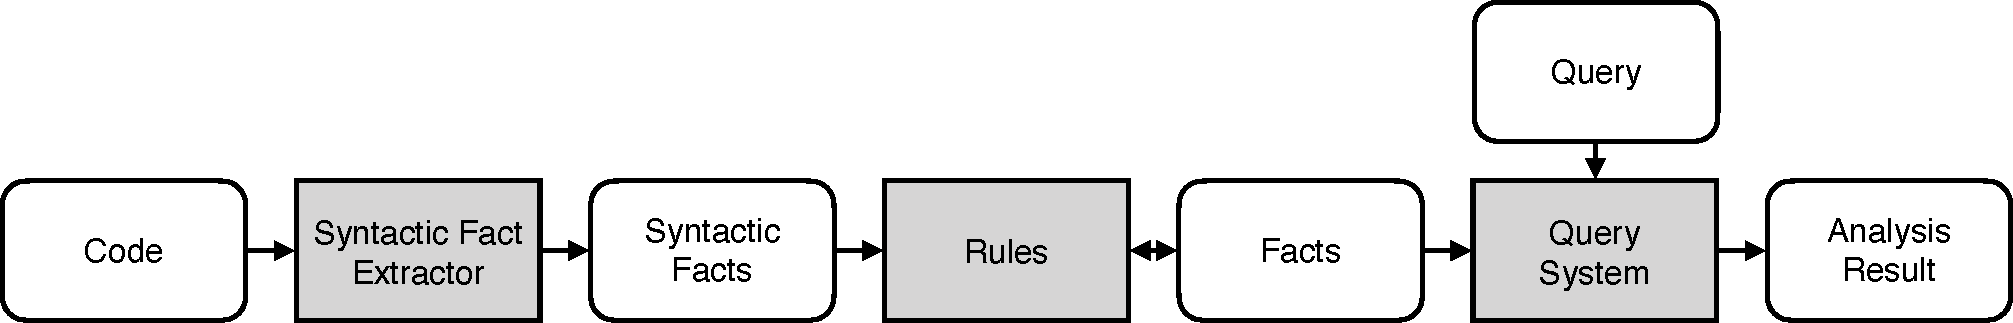
\includegraphics[width=0.94\textwidth]{img/ov1.pdf}
  \caption{Overview of a declarative static analysis}
  \label{fig:ov1}
\end{figure}

Figure~\ref{fig:ov1} presents an overview of how a declarative static
analysis works.  The analysis consists of three steps.  First, a given program
gets converted into syntactic facts. 
\inblue{Second, new facts are generated by iteratively applying rules to the set of
known facts until no new facts are derived.  
Finally, the query system takes a query and evaluates the rules with the given
facts, producing an analysis result for the query. 
The following paragraphs explain each step in detail, with examples written in
the Datalog-like syntax.}

\textbf{Step 1: Extracting syntactic facts.}
The first step is to extract syntactic facts from a given program source.
\inblue{Syntactic facts are the facts that can be statically determined
from the syntax of the given program.}
For example, consider the following code:

\begin{lstlisting}[style=mcpp]
int f() {
  return 42;
}

int val = f();
\end{lstlisting}

\inblue{For function definitions, the Syntactic Fact Extractor can extract syntactic
facts of a form \rcode{ Return(functionName, retExpr)}, where \rcode{Return}
denotes the relation between a string and an expression, \rcode{functionName}
denotes the name of a function, and \rcode{retExpr} denotes the return
expression of the function.
Therefore, the extractor can extract \rcode{ Return("f", 42)} from the
code.  
Another example of syntactic fact is \rcode{ Call(callExpr, functionName)}, which
denotes that \rcode{ callExpr} is a call expression to a function named
\rcode{ functionName}.
For instance, the extractor can extract the following syntactic fact from the
code on line 5: \rcode{ Call(f(), "f")}.}

\smallskip
\inblue{\textbf{Step 2: Deriving new facts by applying rules.}
The next step is to derive new facts from known facts by applying rules.
A rule defines a relation that a fact, called a {\it derivable fact}, can be
derived from a set of facts, called {\it base facts}. 
If all the base facts belong to known facts, the derivable fact is derived and
added to the known facts by the rule.
This process of deriving new facts is repeated until no more new facts are
found.


For example, consider a fact \rcode{ Step(x, y)} that denotes a direct dataflow
from node \rcode{ x} to node \rcode{ y}. 
Here, nodes represent program entities that can hold runtime values,
such as variables, literals, expressions, and function parameters. 
For instance, \rcode{Step(f(), val)} denotes a direct flow from the
result of \rcode{f()} to  \rcode{val}.
A direct dataflow can also be established via the relation between a function call
expression and its callee function's return expression because a function
call expression evaluates to its callee function's return value on runtime.
We can represent such dataflows as the following rule:}
\begin{lstlisting}[style=mrule]
Step(retExpr, callExpr) :- Call(callExpr, functionName), Return(functionName, retExpr)
\end{lstlisting}

\noindent
\inblue{\rcode{Step(retExpr, callExpr)} on the left side of the rule is a derivable
fact, and \rcode{Call(callExpr, functionName)} and \rcode{Return(functionName,
retExpr)} on the right side of the rule are base facts.  
This rule indicates that the new fact \rcode{Step(retExpr, callExpr)} is
derivable if the two base facts are known.
Since we already have \rcode{ Calls(f(), "f")} and \rcode{ Return("f", 42) }
as known facts, the rule derives a new fact \rcode{ Step(42, f()) }.}

\inblue{Derived facts by rules are also known facts used to derive new facts.
For example, we can think of another, \rcode{ Flow(x, z)}, that denotes a
dataflow from node \rcode{ x} to node \rcode{ z}.
We can define rules for the dataflow fact as the transitive closure of \rcode{
  Step}:}

\begin{lstlisting}[style=mrule]
Flow(x, z) :- Step(x, z)
Flow(x, z) :- Step(x, y), Flow(y, z)
\end{lstlisting}

\noindent
\inblue{The first rule indicates that the fact \rcode{ Flow(x, z)} is derivable if the
fact \rcode{ Step(x, z)} is known, and the second rule indicates
that the fact \rcode{ Flow(x, z)} is also derivable if the two facts \rcode{
  Step(x, y)} and \rcode{ Flow(y, z)} are known.
Thus, the rules derive \rcode{ Flow(42, f())}, \rcode{ Flow(f(), val)}, and
\rcode{ Flow(42, val)} from known facts, because \rcode{ Step(42, f())} and
\rcode{ Step(f(), val)} are known.}

\smallskip
\textbf{Step 3: Performing queries.}
The final step is to perform the query via the query system.  
\inblue{A query is a set of facts containing variables, and the query system finds
every variable assignment that makes the facts in the query belong to known
facts.}
This step corresponds to actually obtaining the final result of a static
analysis in a declarative style.  
For example, one can make a specific query:

\begin{lstlisting}[style=mrule]
?- Flow(42, X)
\end{lstlisting}

\noindent
that queries all nodes into which the integer literal {\tt 42} flows.
\inblue{When accepting the query as an input, the query system finds every value
\rcode{ v} such that \rcode{ Flow(42, v)} belongs to known facts generated in
the previous step. 
In this example, the query would give the query result
\rcode{ X\ $\in$ \{f(), val\}}.}

%The final step is to perform queries via query system.
%The result of the query corresponds to actual result of client analysis.
%A query consists of set of facts, where some of the facts would have
%varaibles as arguments. Given a query, the query sytem will find all possible
%assignment on variables, that will make every facts would hold under
%the assignment.
%\newpage
